\chapter{Combined Forecasts}
\bichaptertitle{合成预测}

\audiencebox{Staunch Systems Trader}{This chapter is about combining forecasts from different trading rules, including variations of the same rule, so it's required reading for most staunch systems traders. If you're an asset allocating investor using the single ‘no rule' rule or a semi-automatic trader you can skip ahead to chapter nine.\par\medskip
坚定的系统化交易者\par\medskip
本章讨论的是如何把来自不同交易规则的预测组合起来，其中也包括同一规则的不同变体。因此，对于大多数坚定的系统化交易者来说，这是必读内容。
如果你是使用单一“无规则”规则的资产配置型投资者，或者你是半自动交易者，那么你可以直接跳到第九章。}

LIFE IS SIMPLE WHEN YOU HAVE ONLY ONE TRADING RULE. STRONG positive forecast? Then buy. Negative? Sell. But what if you have multiple rules and they disagree?

当你只有一条交易规则时，事情会很简单。预测值强烈为正？那就买。预测值为负？那就卖。但如果你有多条规则，而且它们彼此意见不一致，又该怎么办？

As you saw in the previous chapter, in late 2009 and 2010 one of my trading rules (the EWMAC trend following rule) had turned bullish on crude oil, but another (Carry) was still bearish (see figures 18 and 19). What should I have done -- buy, sell, or do nothing? Multiple forecasts which disagree aren't conclusive -- you need to create a single combined forecast for every instrument.

正如你在上一章中看到的那样，在 2009 年底和 2010 年期间，我的一条交易规则
（EWMAC 趋势跟踪规则）已经对原油转为看多，但另一条规则
（Carry）仍然保持看空
（见图 18 和图 19）。那我到底该怎么做
--- 买、卖，还是按兵不动？彼此冲突的多个预测本身并不足以给出明确结论
--- 你需要为每个品种构建一个单一的合成预测。

\section*{Chapter overview}
\phantomsection
\addcontentsline{toc}{section}{Chapter overview}
\bisectiontitle{本章概览}

\begin{tabularx}{\textwidth}{@{}p{0.30\textwidth}Y@{}}
\textbf{Combining with forecast weights} & How to use forecast weights to produce a single combined forecast for each instrument. \\
\textbf{Choosing the forecast weights} & Using the handcrafting method to find weights for each trading rule. \\
\textbf{Getting the correct variation} & Making sure the combined forecast has the right expected absolute value by correcting for diversification across the individual forecasts. \\
\textbf{Capping combined forecasts} & Just like the forecast from each trading rule you should limit the size of your combined forecasts. \\
\end{tabularx}

\medskip

\begin{tabularx}{\textwidth}{@{}p{0.30\textwidth}Y@{}}
\textbf{用预测权重进行合成} & 如何用预测权重为每个品种生成一个单一合成预测。 \\
\textbf{选择预测权重} & 如何使用手工构造方法，为每条交易规则找到权重。 \\
\textbf{让波动幅度正确} & 通过修正各个单独预测之间的分散化效应， 确保合成预测拥有正确的预期绝对值。 \\
\textbf{给合成预测设上限} & 就像单条交易规则的预测值一样， 你也应限制合成预测的大小。 \\
\end{tabularx}

\section*{Combining with forecast weights}
\phantomsection
\addcontentsline{toc}{section}{Combining with forecast weights}
\bisectiontitle{用预测权重进行合成}

How do you go from two or more forecasts, to a single combined forecast for each instrument? In the framework you need to use a weighted average of your forecasts, where the weights are forecast weights. These are a type of portfolio weight, where your portfolio consists of trading rule variations, and they should all be positive and add up to 100\%. So if you were trading crude oil in mid-2009, as shown in figures 18 and 19, then you might have had forecasts of +15 in the EWMAC trend following variation and -10 in Carry. With forecast weights of 50\% in each rule your combined forecast would be 2.5.86

你该如何从两个或更多预测值，得到每个品种一个单一的合成预测？在这个框架里，你需要对这些预测值做加权平均，而这些权重就叫预测权重
（forecast weights）。它们本质上是一种投资组合权重，只不过这里的“资产组合”由交易规则变体组成，而且这些权重都应当为正，并且加总为 100\%。
因此，如果你在 2009 年中交易原油，正如图 18 和图 19 所展示的那样，那么你当时可能有一个来自 EWMAC 趋势跟踪变体的 +15 预测值，
以及一个来自 Carry 规则的 -10 预测值。如果这两条规则的预测权重各占 50\%，那么你的合成预测就是 2.5。86

\section*{Choosing the forecast weights}
\phantomsection
\addcontentsline{toc}{section}{Choosing the forecast weights}
\bisectiontitle{选择预测权重}

How do you find the best weights to use when combining forecasts? This is an example of the problem of allocating a portfolio of assets, which we discussed in chapter four. But now the asset weights you have to choose are forecast weights for trading rules and their variations, rather than long positions in equities or bonds.

那么，在组合预测值时，你该如何找到最好的权重？这其实就是我们在第四章讨论过的“资产组合配置”问题的一个实例。
只不过现在你要选择的“资产权重”，不再是股票或债券多头头寸的权重，而是交易规则及其变体的预测权重。

Forecast weights might be the same for all instruments, or different. I'll now show you how to use the handcrafting method I described in chapter four to find those weights, although you can also use bootstrapping if you're comfortable with that.\footnote{Naturally this should be done on an out of sample basis, so your weights change during the back-test. After cost performance must be used when generating portfolio weights. I discuss costs more in chapter twelve, ‘Speed and Size'.\par 当然，这件事应当在样本外基础上完成，
也就是说你的权重会在回测过程中随时间变化。生成投资组合权重时，必须使用扣除成本后的表现数据。关于成本问题，我会在第十二章“速度与规模”中进一步讨论。}
To find handcrafted weights you need both correlations and a way of grouping your assets. You can back-test the performance of different trading rules to get historical estimates for correlations. Alternatively tables 56 and 57 in appendix C (from page 294) give some typical values for trading rules within the same instrument. Once you have correlations the next step in the handcrafted method is to group your assets. The simplest way is to group the variations within a particular trading rule, then allocate across trading rules. Let's take a simple example. Suppose we're using the two rules from the last chapter, trend following (EWMAC) and Carry. For now assume that EWMAC has three variants, with fast look-backs of 16, 32 and 64 for the moving averages.\footnote{The slow look-back is 4 times the fast, as discussed in appendix B, page 284.\par 正如附录 B
第 284 页所讨论的那样，慢均线的回看期是快均线的 4 倍。} The carry rule has a single variation. Here is how I calculated the weights.

预测权重可以对所有品种都相同，也可以因品种而异。现在我来展示如何使用第四章中介绍过的手工构造方法，来找到这些权重，
当然，如果你对 bootstrapping 足够熟悉，也可以使用它。要找出手工构造权重，你既需要相关性信息，也需要一种对“资产”进行分组的方法。
你可以通过回测不同交易规则的表现，来得到历史相关性的估计。另一种方法，是使用附录 C 中表 56 和表 57
（第 294 页起）给出的同一品种内不同交易规则的一些典型数值。一旦得到相关性，手工构造法的下一步就是对这些“资产”进行分组。
最简单的方法，是先在某条特定交易规则内部对不同变体分组，然后再在不同交易规则之间做配置。我们来看一个简单的例子。
假设我们使用上一章里的两条规则：趋势跟踪
（EWMAC）和 Carry。先假设 EWMAC 有三个变体，它们的快均线回看期分别为 16、32 和 64。Carry 规则则只有一个变体。
下面是我计算这些权重的方式。

First level • Group one (EWMAC): From table 57 in appendix C (page 295) I get grouping the correlations between EWMAC variations: 0.90 between adjacent Within trading variations, and 0.7 between the variations with fast look-backs 16 and rules 64. Using table 8 (page 79) row 11 I get weights of 16\% in look-back 32, and 42\% in look-backs 16 and 64. • Group two (Carry): One asset. Using table 8 row 1: 100\% in Carry.

第一层分组
• 第一组（EWMAC）：
从附录 C 的表 57
（第 295 页）中，我得到 EWMAC 各变体之间的相关性：相邻变体之间为 0.90，而快回看期为 16 和 64 的两个变体之间为 0.7。
使用表 8
（第 79 页）的第 11 行，我得到的权重是：回看期为 32 的变体占 16\%，而回看期为 16 和 64 的两个变体各占 42\%。
• 第二组（Carry）：
只有一个“资产”。使用表 8 第 1 行：Carry 权重为 100\%。

Second level Using table 8 row 2: 50\% in the EWMAC and 50\% in Carry. grouping Across trading rules

第二层分组
使用表 8 第 2 行：EWMAC 占 50\%，Carry 占 50\%。

This gives us the weights in table 17. By the way it's also possible to have a three level grouping, if you are mixing rules of different styles.

这样我们就得到了表 17 中的权重。顺便一提，如果你混合使用不同风格的规则，那么也可以有三层分组结构。

\rawtablecaption{EXAMPLE HANDCRAFTED FORECAST WEIGHTS\\手工构造预测权重示例}
\begingroup
\small
\centering
\begin{tabular}{@{}lrrr@{}}
\toprule
& 1st level & 2nd level & Final weights \\
\midrule
EWMAC 16, 64 & 42\% & 50\% & 21\% \\
EWMAC 32, 128 & 16\% & 50\% & 8\% \\
EWMAC 64, 256 & 42\% & 50\% & 21\% \\
Carry & 100\% & 50\% & 50\% \\
\bottomrule
\end{tabular}
\par
\endgroup

\begingroup
\small
\centering
\begin{tabular}{@{}lrrr@{}}
\toprule
& 第一层权重 & 第二层权重 & 最终权重 \\
\midrule
EWMAC 16, 64 & 42\% & 50\% & 21\% \\
EWMAC 32, 128 & 16\% & 50\% & 8\% \\
EWMAC 64, 256 & 42\% & 50\% & 21\% \\
Carry & 100\% & 50\% & 50\% \\
\bottomrule
\end{tabular}
\par
\endgroup

Notice that I haven’t shown you how to incorporate different performance between rules,
the effect of costs, or how to decide if different instruments should have different weights.
If you’ve followed my advice from chapter three, and not fitted or selected trading rules
based on Sharpe ratio, then you risk having some poor rules in your portfolio, on which
you could want to reduce the allocation. It’s also quite likely faster rules will have worse
after-cost performance than slower ones.
I’ll discuss these issues in detail in chapter twelve, ‘Speed and Size’. There will also be
a more realistic example using performance and cost estimates in the staunch systems
trader example chapter in part four.

请注意，我这里还没有向你展示如何把不同规则之间的表现差异纳入考虑，
也没有展示成本效应，或者如何决定不同品种是否应当拥有不同权重。
如果你遵循了我在第三章中的建议，没有根据夏普比率去拟合或筛选交易规则，
那么你的投资组合里就可能包含一些质量较差的规则，而你也许会想减少它们的配置。
同时，更快的规则在扣除成本后，其表现也很可能比更慢的规则更差。
我会在第十二章“速度与规模”中详细讨论这些问题。
在本书第四部分“坚定的系统化交易者”示例章节中，
我还会给出一个更贴近现实的例子，其中会使用表现和成本估计值。

\section*{Getting to 10}
\phantomsection
\addcontentsline{toc}{section}{Getting to 10}
\bisectiontitle{把平均绝对值拉回到 10}

I recommended in chapter six that all your individual forecasts should have the same expected variability -- equivalent to an expected absolute value of 10. But unless your trading rules are perfectly correlated it's likely that the combined forecast will end up on a smaller scale. It's the same general effect you get from putting less than perfectly correlated assets into any portfolio, where the overall portfolio will always end up with lower risk than its constituents. The magnitude of the fall in standard deviation will depend on the degree of diversification. However the trading system framework will not work consistently if combined forecasts have a low and unpredictable scaling. You need your combined forecasts to maintain the same expected absolute value of 10 as you required for individual forecasts. To fix this the combined forecast is multiplied by a forecast diversification multiplier.

我在第六章中建议，所有单独预测值都应当具有相同的预期波动幅度
--- 也就是预期绝对值平均为 10。但除非你的交易规则彼此完全相关，否则合成预测值很可能会缩小到一个更小的尺度。
这和任何投资组合中把相关性不完全相同的资产放在一起时所发生的效应是一样的：整体投资组合的风险总会低于其组成部分的风险。
标准差下降的幅度，取决于分散化程度。然而，如果合成预测值的尺度既偏低又不可预测，那么整个交易系统框架就无法稳定地工作。
你需要让合成预测值保持与单个预测值相同的预期绝对值 10。为了解决这个问题，必须把合成预测值乘以一个预测分散化乘数
（forecast diversification multiplier）。

CONCEPT: DIVERSIFICATION MULTIPLIER If you have two stocks, each with identical return volatility of 10\%, with half your money in each, what will be the volatility of the whole portfolio? Naturally it will depend on how correlated the two assets are. If they are perfectly correlated then the portfolio will have a return standard deviation of 10\%; the same as the individual assets. But if the correlation between the two assets was 0.5, the portfolio volatility would come out at 8.66\%.89 Similarly a correlation of zero gives a volatility of 7.07\%. More diversified portfolios have lower volatility. In the framework we are concerned with putting together volatility standardised assets that have the same expected average standard deviation of returns; and to do this we need forecasts to have the same average absolute value. To ensure this is always the case you need to multiply the forecasts or positions you have to account for portfolio diversification, so that your total portfolio also achieves the standard volatility target. This multiplication factor is the diversification multiplier.90 If the correlation between the two assets in the simple two stocks example is 1.0, then because the portfolio has the same volatility as its members (10\%) no adjustment is required, and the multiplier will be 1. A correlation of 0.5 implies a multiplier equal to the target volatility of 10\%, divided by the natural portfolio volatility of 8.66\%. This will be 10 ÷ 8.66 = 1.15. Finally if the two assets were completely uncorrelated with portfolio volatility of 7.07\%, then the multiplier would be 10 ÷ 7.07 = 1.44. You will get even higher values with negative correlations. However this will result in dangerously large multipliers, so I strongly recommend you floor any estimated correlations at zero. You can use two possible sources for correlations to do this calculation. Correlations can be estimated with data from back-tests, or using rule of thumb values from the tables in appendix C.91 You can do the actual calculation with the precise equation, or alternatively table 18 gives a rule of thumb which will give a good approximation.92

概念：分散化乘数 假设你有两只股票，它们的收益波动率完全相同，都是 10\%，而你把一半资金放在每一只股票上，
那么整个组合的波动率是多少？显然，这取决于这两项资产之间的相关性。如果它们完全相关，那么整个投资组合的收益标准差就是 10\%，
与单个资产相同。但如果这两项资产之间的相关性是 0.5，那么组合波动率就会变成 8.66\%。89 同样地，如果相关性是 0，
那么波动率就是 7.07\%。分散化程度越高，投资组合的波动率就越低。在这个框架里，我们关心的是如何把已经完成波动率标准化、并且具有相同预期平均收益标准差的“资产”放在一起；
而要做到这一点，我们就需要让预测值也具有相同的平均绝对值。为了确保这一点始终成立，你就必须对预测值或仓位施加一个乘数，
用来修正投资组合中的分散化效应，从而让整个投资组合也能够达到标准的波动率目标。这个乘数，就是分散化乘数。90
在刚才两只股票的简单例子中，如果两项资产的相关性为 1.0，那么由于投资组合的波动率与组成成员相同
（都是 10\%），就不需要做任何调整，因此乘数是 1。如果相关性为 0.5，那么乘数就等于目标波动率 10\% 除以组合的天然波动率 8.66\%，
也就是 10 ÷ 8.66 = 1.15。最后，如果这两项资产完全不相关，而组合波动率是 7.07\%，那么乘数就会变成 10 ÷ 7.07 = 1.44。
如果相关性是负的，这个值还会更高。然而，这会带来危险地过大的乘数，所以我强烈建议你把所有估计出的负相关都先截断为 0。
要完成这一计算，你有两个可能的数据来源。相关性可以通过回测数据来估计，也可以使用附录 C 表格中的经验法则数值。91
至于实际计算，你可以用精确公式来做；或者，也可以使用表 18 中给出的经验近似值，它已经相当准确。92

\begin{enumerate}
  \item You can replicate this result with one of the many online portfolio calculators, such as www.zenwealth. com/businessfinanceonline/RR/PortfolioCalculator.html
  \item The diversification multiplier is also a measure of the number of independent bets in the portfolio, as used in the law of active management.
  \item A couple of technical points. Firstly strictly speaking diversification multipliers should be calculated on a rolling out of sample basis if based on back-tested data. However as you're not optimising a parameter based on profitability, estimating these single multipliers won't cause serious problems with over-fitting. Secondly when estimating forecast diversification multipliers you can either use the forecasts from each individual instrument, or pool back-tests of different instruments (which is my preferred approach), before calculating correlation matrices.
\end{enumerate}

\begin{enumerate}
  \item 你可以用众多在线投资组合计算器中的任意一个复现这个结果，例如 `www.zenwealth.com/businessfinanceonline/RR/PortfolioCalculator.html`。
  \item 分散化乘数也可以被视为组合中“独立下注数量”的一种度量，这正是主动管理定律中的一个概念。
  \item 还有两个技术性提醒。第一，严格来说，如果你是根据回测数据来计算分散化乘数，那么它应当在滚动样本外基础上进行计算。
  不过由于你并不是基于盈利能力去优化某个参数，因此估计这种单一乘数并不会带来严重的过拟合问题。第二，在估计预测分散化乘数时，
  你既可以使用每个单独品种自身的预测值，也可以先把不同品种的回测结果合并起来
  （这是我更偏好的方法），然后再去计算相关矩阵。
\end{enumerate}

\begin{figure}[htbp]
  \centering
  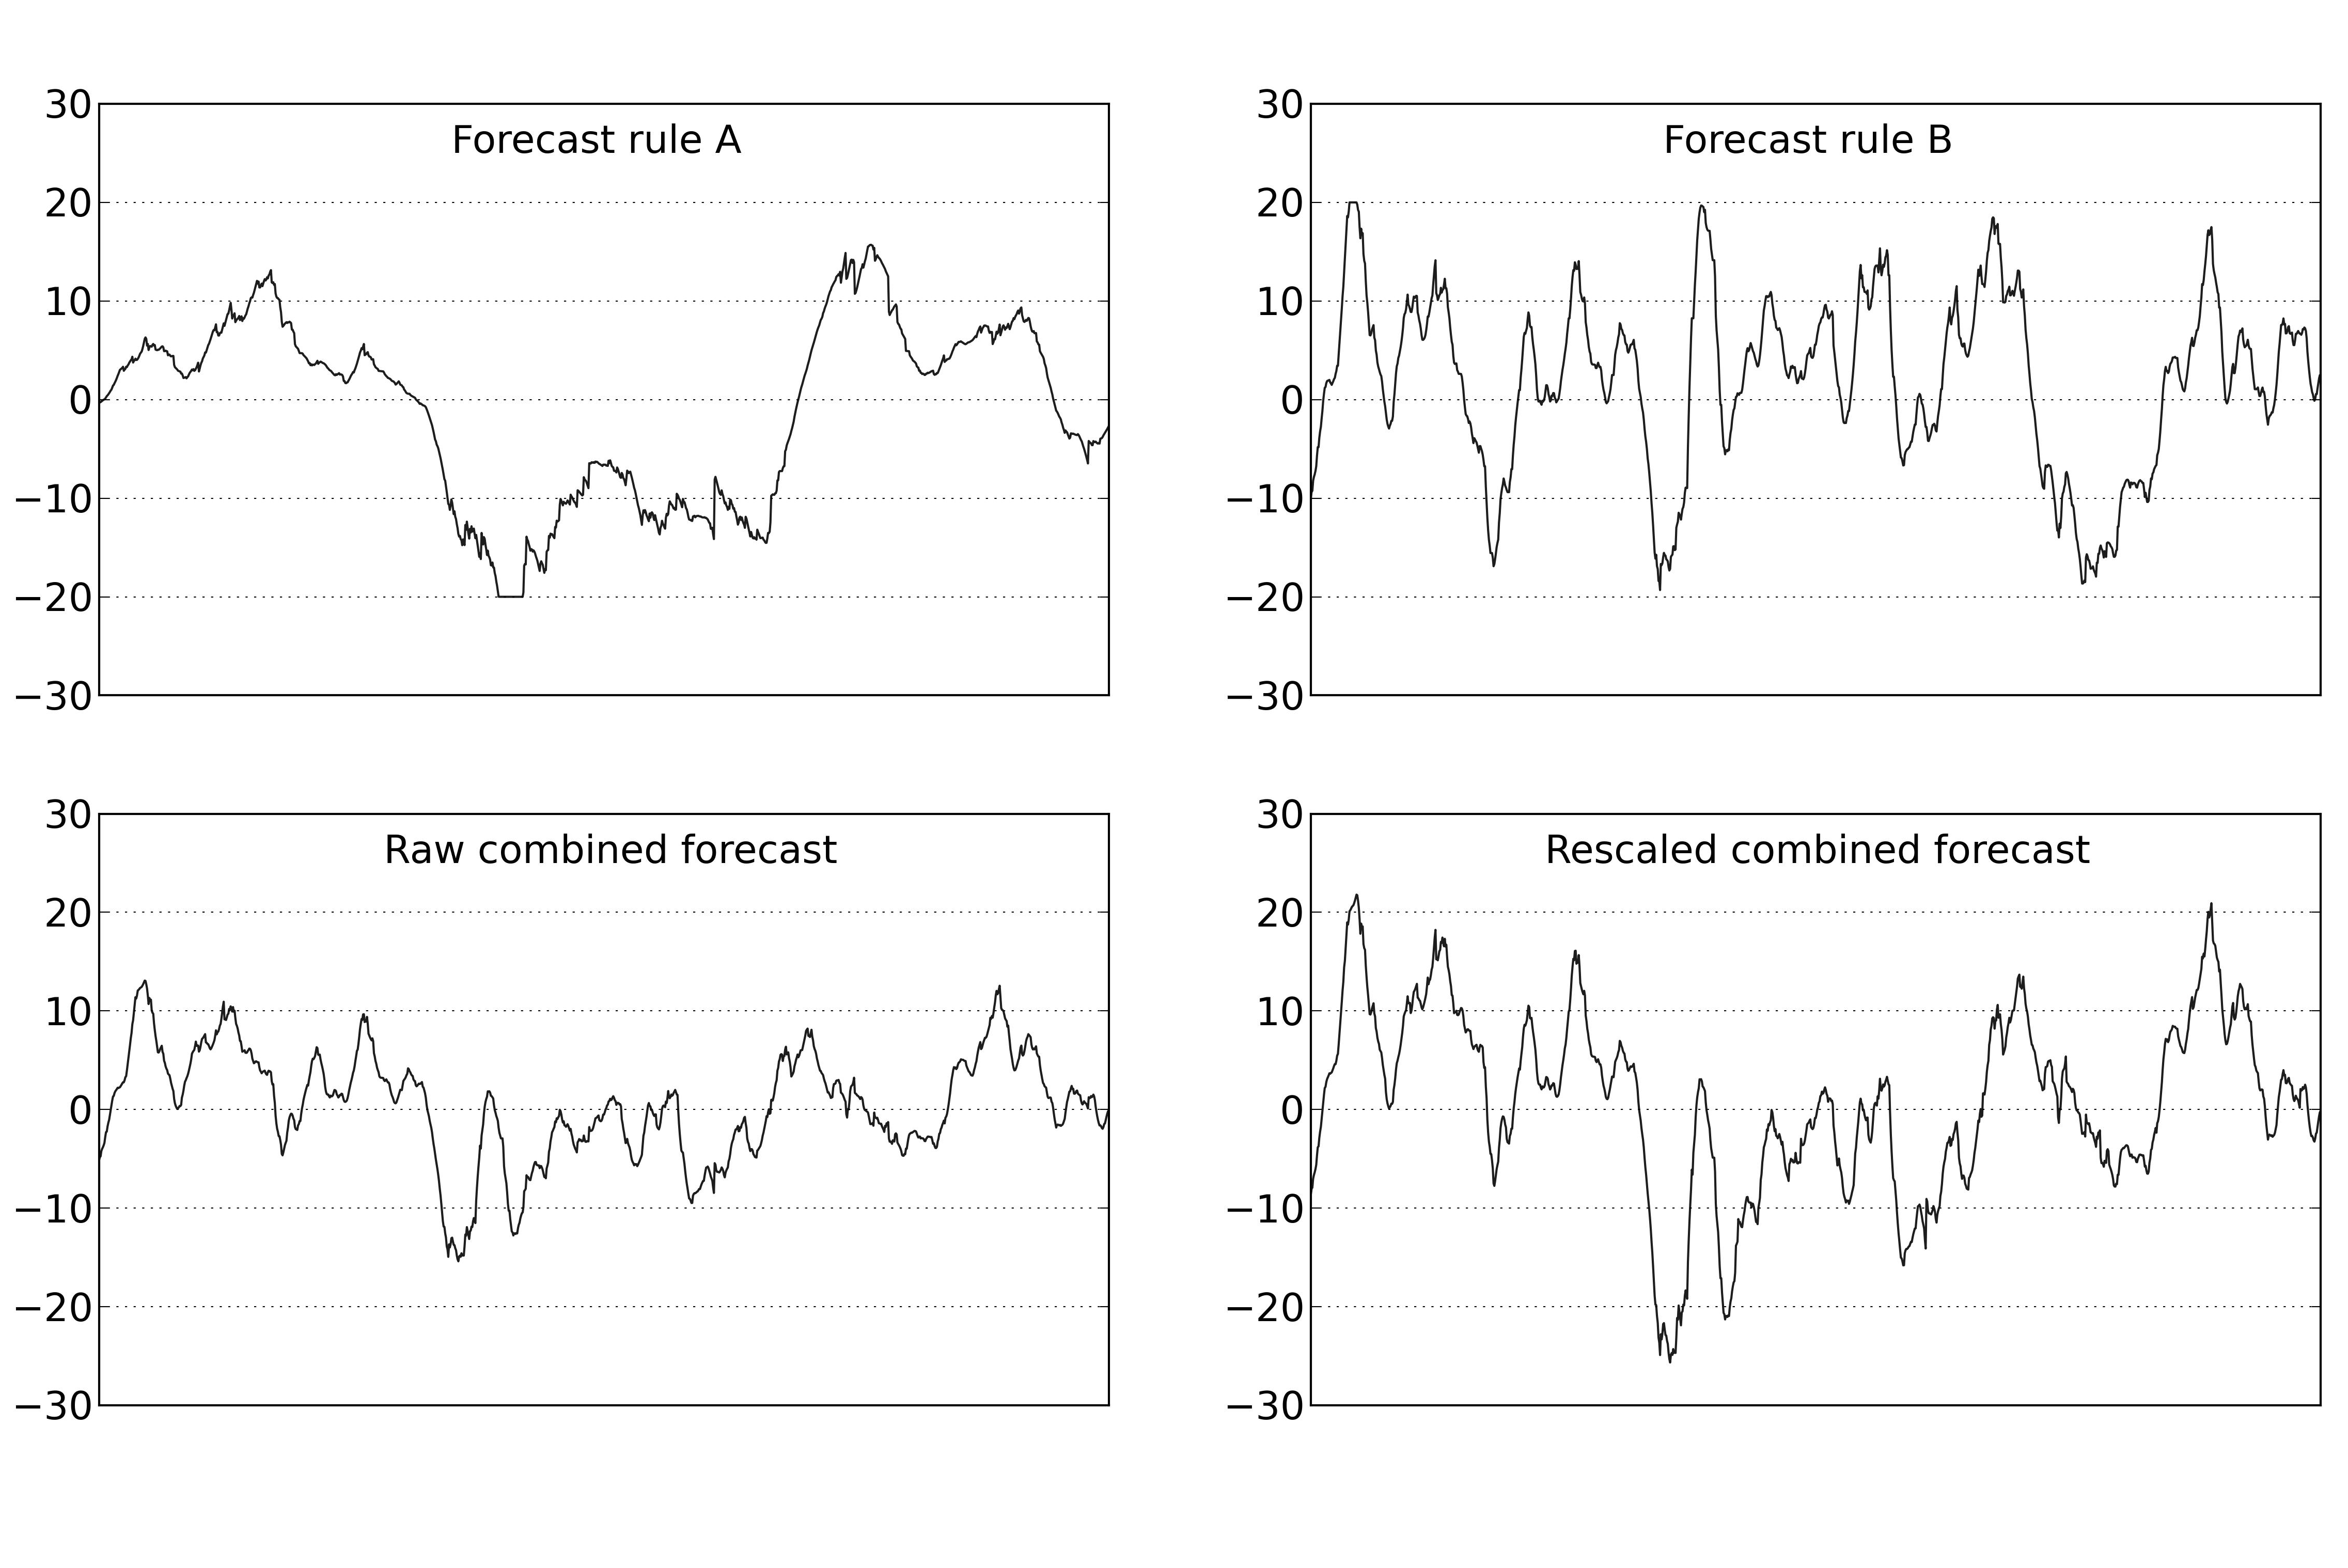
\includegraphics[width=\textwidth]{figures/raw/img-020.png}
  \caption{COMBINING DIFFERENT FORECASTS REDUCES VARIABILITY. RESCALING FIXES THIS\\
  把不同预测值组合在一起会降低波动幅度，而重缩放可以修正这个问题}
\end{figure}

Figure 20 shows this effect for two uncorrelated forecasts A and B, which I've combined with a 50\% weight to each. They cover the range from -20 to +20. But the combined forecast is much less variable than I want, with a smaller range of -15 to +12. Scaling the combined forecast up with a forecast diversification multiplier fixes the problem.

图 20 展示了这一效应：我把两个互不相关的预测 A 和 B 按各 50\% 的权重进行组合。它们各自都覆盖从 -20 到 +20 的区间。
但组合之后的预测值波动幅度明显比我想要的小，结果只落在 -15 到 +12 之间。把合成预测值乘上预测分散化乘数进行放大之后，这个问题就被修正了。

\rawtablecaption{MORE ASSETS AND LOWER CORRELATIONS MEAN MORE DIVERSIFICATION AND A HIGHER MULTIPLIER93\\更多资产与更低相关性意味着更强分散化和更高乘数93}
\begingroup
\small
\centering
\begin{tabular}{@{}rccccc@{}}
\toprule
\textbf{Number of assets} & \multicolumn{5}{c}{\textbf{Average correlation between assets}} \\
\cmidrule(l){2-6}
& 0.0 & 0.25 & 0.5 & 0.75 & 1.0 \\
\midrule
2 & 1.41 & 1.27 & 1.15 & 1.10 & 1.0 \\
3 & 1.73 & 1.41 & 1.22 & 1.12 & 1.0 \\
4 & 2.0 & 1.51 & 1.27 & 1.10 & 1.0 \\
5 & 2.2 & 1.58 & 1.29 & 1.15 & 1.0 \\
10 & 3.2 & 1.75 & 1.35 & 1.17 & 1.0 \\
15 & 3.9 & 1.83 & 1.37 & 1.17 & 1.0 \\
20 & 4.5 & 1.86 & 1.38 & 1.18 & 1.0 \\
50 or more & 7.1 & 1.94 & 1.40 & 1.19 & 1.0 \\
\bottomrule
\end{tabular}
\par
\endgroup

\begingroup
\small
\centering
\begin{tabular}{@{}rccccc@{}}
\toprule
\textbf{资产数量} & \multicolumn{5}{c}{\textbf{资产之间的平均相关性}} \\
\cmidrule(l){2-6}
& 0.0 & 0.25 & 0.5 & 0.75 & 1.0 \\
\midrule
2 & 1.41 & 1.27 & 1.15 & 1.10 & 1.0 \\
3 & 1.73 & 1.41 & 1.22 & 1.12 & 1.0 \\
4 & 2.0 & 1.51 & 1.27 & 1.10 & 1.0 \\
5 & 2.2 & 1.58 & 1.29 & 1.15 & 1.0 \\
10 & 3.2 & 1.75 & 1.35 & 1.17 & 1.0 \\
15 & 3.9 & 1.83 & 1.37 & 1.17 & 1.0 \\
20 & 4.5 & 1.86 & 1.38 & 1.18 & 1.0 \\
50 或更多 & 7.1 & 1.94 & 1.40 & 1.19 & 1.0 \\
\bottomrule
\end{tabular}
\par
\endgroup

The table shows the approximate diversification multiplier given the number of assets in a portfolio (rows) and the average correlation between them (columns). Beware of using very high multipliers.

这张表展示的是：在给定投资组合中资产数量
（行）以及它们之间平均相关性
（列）的情况下，分散化乘数的大致取值。请务必警惕使用过高的乘数。

I'll now explain how to calculate the forecast diversification multiplier. If you don't have back-tested forecast values then you can estimate likely correlations from tables 56 and 57 in appendix C (from page 294). Correlation between selected variations of the same rule tends to be high; up to 0.9 but averaging around 0.7. Across different trading rules within the same style it is around 0.5. Using different styles of rules, correlations for trading rules within an instrument are around 0.25. For the simple example with four rule variations from earlier in the chapter I populated a correlation matrix using the information in appendix C, which is shown in table 19.

下面我来解释如何计算预测分散化乘数。如果你没有回测得到的预测值，那么你可以利用附录 C 中表 56 和表 57
（从第 294 页开始）来估计相关性的合理范围。同一条规则中所选变体之间的相关性通常很高，最高可达 0.9，平均大约在 0.7 左右。
同一风格下的不同交易规则之间，相关性大约在 0.5 左右。若使用不同风格的规则，那么同一品种内部不同交易规则之间的相关性大约在 0.25。
对于本章前面那个包含四个规则变体的简单例子，我利用附录 C 的信息构造了一个相关矩阵，如表 19 所示。

\rawtablecaption{CORRELATION OF TRADING RULE FORECASTS IN SIMPLE EXAMPLE\\简单示例中交易规则预测值的相关性}
\begingroup
\small
\centering
\begin{tabular}{@{}lcccc@{}}
\toprule
& EW16 & EW32 & EW64 & Carry \\
\midrule
EWMAC 16,64 & 1 & & & \\
EWMAC 32,128 & 0.9 & 1 & & \\
EWMAC 64,256 & 0.6 & 0.9 & 1 & \\
Carry & 0.25 & 0.25 & 0.25 & 1 \\
\bottomrule
\end{tabular}
\par
\endgroup

\begingroup
\small
\centering
\begin{tabular}{@{}lcccc@{}}
\toprule
& EW16 & EW32 & EW64 & Carry \\
\midrule
EWMAC 16,64 & 1 & & & \\
EWMAC 32,128 & 0.9 & 1 & & \\
EWMAC 64,256 & 0.6 & 0.9 & 1 & \\
Carry & 0.25 & 0.25 & 0.25 & 1 \\
\bottomrule
\end{tabular}
\par
\endgroup

Values shown are correlations, populated using values in appendix C tables.

You could now use tables 18 and 19 to find an approximate forecast diversification
multiplier for the four rule variations. The matrix in table 19 has a rounded average
correlation of 0.50,94 which with four assets in table 18 gives a multiplier of 1.27. As a
comparison the precise value is 1.31 using the actual forecast weights calculated above
and the formula on page 297.
Finally, a word of warning. It’s possible, as table 18 shows us, to get very high multipliers
if your trading rules are sufficiently diversified, even if you cap negative correlations at
zero. As you’ll see in a moment I recommend that combined forecasts are limited to a
maximum value of 20, so having a high multiplier would mean having capped forecasts
most of the time, and effectively behaving as if you had a binary trading rule which is
either fully long or fully short.
To avoid this I advocate using a maximum diversification multiplier of 2.5, regardless of
what your actual estimate is.

表中所示为相关性，使用附录 C 各表中的数值填充得到。

现在你可以结合表 18 和表 19，找出这四个规则变体的大致预测分散化乘数。
表 19 中相关矩阵的平均相关性大约为 0.50。94
在表 18 中，四个“资产”对应的乘数约为 1.27。作为比较，
若使用上文算出的实际预测权重以及第 297 页中的公式，
得到的精确值是 1.31。
最后，提醒一句。正如表 18 所展示的那样，
如果你的交易规则足够分散，即便你已经把负相关截断为 0，
仍然有可能得到非常高的乘数。
你很快会看到，我建议把合成预测值限制在最大 20 的范围内，
因此，如果乘数过高，就意味着你的预测值在大多数时候都会被封顶，
最终整个系统会表现得像一条二元交易规则一样：
要么全多，要么全空。
为了避免这种情况，我建议无论你的实际估计值是多少，
都把分散化乘数的最大值限制为 2.5。

\section*{Capped at 20}
\phantomsection
\addcontentsline{toc}{section}{Capped at 20}
\bisectiontitle{封顶在 20}

In the previous chapter I recommended that you limit the forecast from individual rules to the range -20 to +20. However it's possible in theory for a combined forecast to go above 20 if the forecast diversification multiplier is greater than 1, as is usually the case. To take a simple example, if the Carry rule and a single EWMAC variation both had forecasts of +16, with forecast weights of 50\% on each rule, and a diversification multiplier of 1.5, then the combined forecast would be 24.95

在上一章中，我建议把每条单独规则的预测值限制在 -20 到 +20 之间。然而，理论上来说，只要预测分散化乘数大于 1
--- 而这通常都会发生
--- 那么合成预测值就有可能超过 20。举个简单的例子，如果 Carry 规则和某个单独的 EWMAC 变体都给出了 +16 的预测值，
且这两条规则的预测权重各为 50\%，分散化乘数又是 1.5，那么合成预测值就会达到 24。95

All the reasons cited in the previous chapter for limiting individual forecasts apply equally to combined forecasts, so I strongly encourage you to limit combined forecasts to absolute values of 20 or less. Any value outside this range should be capped.

上一章中列出的所有“为什么要限制单个预测值”的理由，同样也适用于合成预测值。因此，我强烈建议你也把合成预测值限制在绝对值不超过 20 的范围内。
任何超出这个区间的值，都应当被封顶。

\section*{Summary for combining forecasts}
\phantomsection
\addcontentsline{toc}{section}{Summary for combining forecasts}
\bisectiontitle{合成预测总结}

Instrument You start with the forecasts for each trading rule variation for an instrument. forecasts for So if you have two rules, each with three variations, then you'd have six each trading possible forecast values per instrument. rule and I recommended in the previous chapter that each individual forecast has variation an expected average absolute value of around 10 and should be limited to between -20 and +20.

品种预测值 你从某个品种在每个交易规则变体下的预测值开始。如果你有两条规则，每条规则又各有三个变体，那么每个品种就会有六个可能的预测值。
我在上一章中建议，每个单独预测值的预期平均绝对值应当大约为 10，并限制在 -20 到 +20 之间。

Forecast Each rule variation should have a positive forecast weight. The weights weights must add up to 100\%. These weights can be the same across instruments, or different.

预测权重 每个规则变体都应当有一个正的预测权重。所有权重必须加总为 100\%。这些权重可以在不同品种之间相同，也可以不同。

Raw combined Using the forecast weights, take a weighted average of the forecasts from forecast each rule variation.

原始合成预测 使用预测权重，对各个规则变体的预测值做加权平均。

Forecast This is needed to get the expected absolute value of the combined forecast diversification up to the recommended value of 10. multiplier Estimated correlations are needed; from back-test results, or the rule of thumb tables in appendix C. You can then calculate the multiplier approximately from table 18 or precisely using the equation on page 297. The multiplier is at least 1.0 and I recommend a maximum of 2.5.

预测分散化乘数 你需要它，才能把合成预测值的预期绝对值拉回到建议值 10。为此你需要相关性估计，它可以来自回测结果，
也可以来自附录 C 中的经验表格。然后，你可以利用表 18 粗略计算乘数，或者使用第 297 页的公式进行精确计算。乘数至少为 1.0，
而我建议它的最大值不要超过 2.5。

Rescaled This is the raw combined forecast multiplied by the forecast diversification combined multiplier. forecast Because of the diversification multiplier it will have an expected average absolute value equal to the expected variability of the individual forecasts, which I recommend to be 10.

重缩放后的合成预测 这等于原始合成预测乘以预测分散化乘数。正因为有这个乘数，它的预期平均绝对值才会与单独预测值的预期波动幅度一致，
而我建议这个值应为 10。

Final combined I recommend you cap the rescaled combined forecasts within the range forecast -20 to +20, as for individual forecasts.

最终合成预测 我建议你像处理单独预测值一样，把重缩放后的合成预测也限制在 -20 到 +20 的区间内。

Now you can forecast price movements for a particular instrument you are ready to translate that into actual trades. The first step in doing this is to decide how much money you are willing to put at risk, as you'll see in the next chapter.

现在，你已经能够为某个具体品种预测价格走势，也就准备好把它转换成实际交易了。而要做到这一点，第一步就是决定你愿意承担多大金额的风险，
正如你会在下一章中看到的那样。
